\ADComment{Please ignore my comments in this section for now.}

We now present \emph{static pairwise lockset analysis}, a novel method for data race analysis in concurrent device drivers.
In Section~\ref{ } we explain conceptually how the approach works.
In Section~\ref{ } we describe our implementation of static pairwise lockset analysis in a practical tool,
Whoop, that can be applied directly to driver source code, to check whether pairs of driver entry points are 
free from data races.

We demonstrate in Section~\ref{ } both that the Whoop technique and tool has value in its own right as a stand-alone static analyser, and that results from Whoop can be exploited to significantly boost performance of a more precise static analysis for concurrency offered by the CORRAL tool, based on context bounding and stratified inlining.

\subsection{Static pairwise lockset analysis}

\ADComment{Ally: first, let us try to explain really clearly in words how the technique works.}

\ADComment{Second, let's introduce some notation to describe the thing more formally.}

\ADComment{Finally, try to set up some kind of theorem giving the guarantee we think we have.}



\subsection{Implementation in Whoop}





The entry points for 



We have implemented our approach in \whoop, a static lockset analysis infrastructure that uses state-of-the-art compilation and sequential verification techniques to (i) automatically analyze Linux drivers for potential data races and (ii) exploit the race-related information from the sound static analysis phase to accelerate bug-finding.

\begin{figure*}
\centering
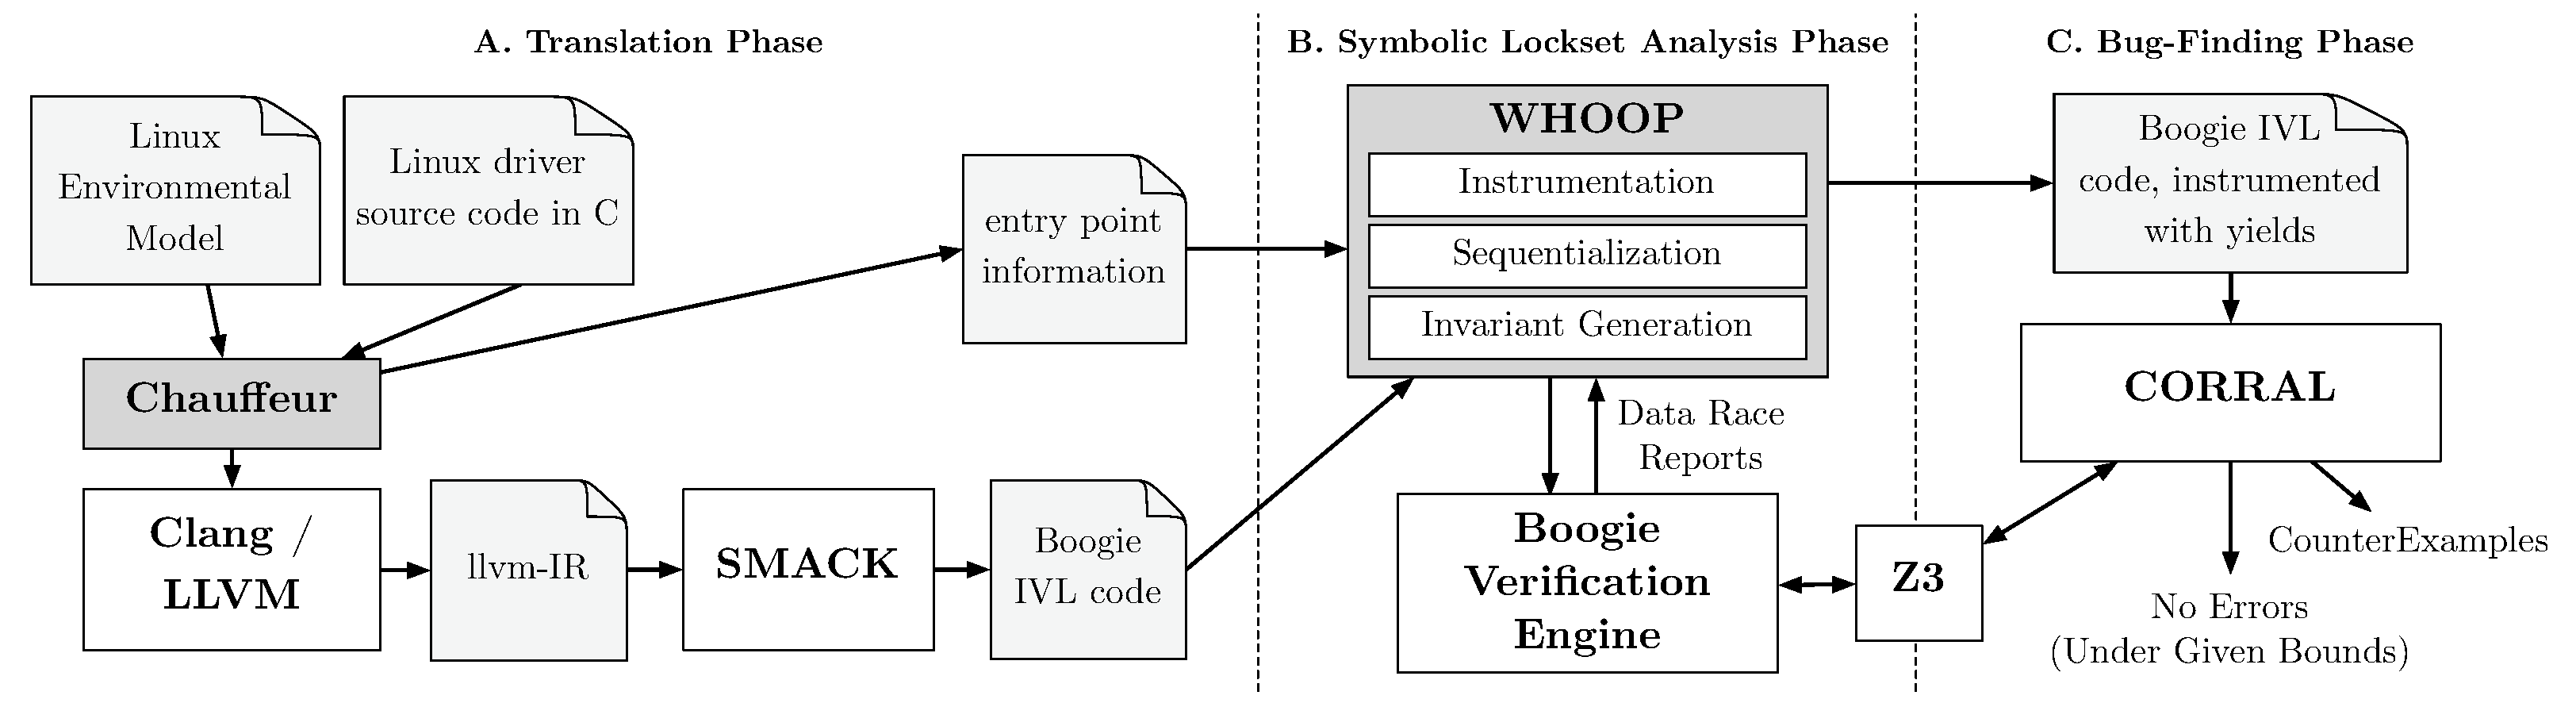
\includegraphics[width=.99\linewidth]{img/whoop.pdf}
\caption{The \whoop infrastructure, empowered by state-of-the-art compilation (Clang/LLVM and SMACK) and verification (Boogie and \corral) tools}
\label{fig:whoop}
\end{figure*}

The key idea behind our novel static analysis is that we can verify absence of data races by (i) deriving a sound \emph{sequential} model that \emph{over-approximates} the originally concurrent program, (ii) instrumenting it for lockset analysis and race-checking, and (iii) asserting that all write/read accesses to the same shared resource are consistently protected by at least one common lock. The immediate benefit is that our approach not only avoids reasoning about thread interleavings, and thus has the potential to scale well, but also allows the reuse of existing sequential verification techniques.

Figure~\ref{fig:whoop} depicts the \whoop toolchain. Initially, \whoop accepts a Linux driver written in C, together with a Linux environmental model\footnote{Stub header files that model the Linux kernel APIs.}, which is required to ``close'' the driver and allow it to be subsequently over-approximated and analyzed. Both the driver and the environmental model are passed to the translation phase of \whoop (see Section~\ref{whoop:translation}), which outputs an over-approximated program written in the Boogie intermediate verification language (IVL)~\cite{deline2005boogiepl}. Next, \whoop performs \emph{static pairwise lockset analysis} to detect all potential data races in the abstract program. The proof sketch behind our static lockset analysis is given in Section~\ref{whoop:proof}. The instrumentation and analysis is described in more detail in Section~\ref{whoop:method}. The summarization that we perform to achieve scalability is presented in Section~\ref{whoop:summarization}. After the static lockset analysis phase, \whoop exploits the race-related information to accelerate bug-finding with \corral (see Section~\ref{whoop:bugfinding})

Finally, we discuss optimizations and assumptions in Section~\ref{whoop:optimizations}, and limitations of our technique in Section~\ref{whoop:limitations}.

\subsection{Translation to Boogie IVL}
\label{whoop:translation}

The aim of this phase (see Figure~\ref{fig:whoop} -- A) is to take an input Linux driver written in C, together with an environmental model, and output an over-approximated version of the program in Boogie IVL, a simple imperative language with well-defined verification-focused semantics used as the input to a number of cutting-edge verifiers (e.g. Boogie and \corral). To achieve this translation, \whoop uses three LLVM\footnote{http://llvm.org}-based tools: Chauffeur\footnote{https://github.com/mc-imperial/chauffeur}, Clang\footnote{http://clang.llvm.org} and SMACK\footnote{https://github.com/smackers/smack}~\cite{rakamaric2014smack}.

First, \whoop runs Chauffeur, a Clang-frontend that we developed to perform two tasks: (i) visit the abstract syntax tree (AST) of the original program and extract all available entry point identifier names in the given driver, together with the identifier names of their corresponding kernel callbacks; and (ii) instrument the original program with a function that calls all available entry points. This function acts as the main entry point to the driver after the latter has been registered with the kernel. This simple rewriting does not alter the semantics of the original program, is required so that Clang does not compile away any uncalled entry points (because we closed the environment using stub functions) and is also later used by \whoop to help instrument asynchronous calls to entry points and create checker procedures (see Sections~\ref{whoop:method} and~\ref{whoop:bugfinding}). The output is a file that contains information regarding the entry points and a file with the rewritten program.

Next, the rewritten program is passed to Clang which compiles it to LLVM-IR~\cite{lattner2004llvm}, a low-level assembly-like language in single static assignment (SSA) form. SMACK then translates the LLVM-IR to Boogie IVL. SMACK leverages the pointer-alias analyses of LLVM to efficiently model the heap manipulation operations of the original program in Boogie IVL. To achieve scalability, SMACK is using a split-memory model instead of a monolithic one that would be difficult for backend verifiers to reason about~\cite{rakamaric2009scalable}.

\begin{lstlisting}[caption = Simple networking entry point in C, label = fig:original_program]
static void ep1(struct net_device *dev) {
  struct shared *tp = netdev_priv(dev);
  mutex_lock(&tp->wk.mutex);
  tp->resource = 4;
  mutex_unlock(&tp->wk.mutex);
}
\end{lstlisting}

Example~\ref{fig:original_program} shows a simple program in C and Example~\ref{fig:smack_translation} shows its corresponding translation in Boogie IVL using SMACK. The function \texttt{\$pa} models pointer arithmetic, while the map \texttt{\$M.0} is a memory region that typically denotes a shared resource. Notice that function calls (e.g. to lock and unlock a mutex) are preserved in the translation.

\begin{boogie}[caption = Translation to Boogie IVL using SMACK, label = fig:smack_translation]
procedure ep1(dev: int) modifies $M.0; {
  var $p0, $p1, $p2, $p3, $p4, $p5, $p6: int;
  $bb0:
    $p0 := dev;
    $p1 := $pa($p0, 32, 1);
    $p2 := $pa($pa($p1, 0, 24), 12, 1);
    $p3 := $pa($pa($p2, 0, 12), 0, 1);
    call mutex_lock($p3);
    $p4 := $pa($pa($p1, 0, 24), 4, 1);
    $M.0[$p4] := 4;
    $p5 := $pa($pa($p1, 0, 24), 12, 1);
    $p6 := $pa($pa($p5, 0, 12), 0, 1);
    call mutex_unlock($p6);
    return;
}
\end{boogie}

\subsection{Static Lockset Analysis Proof Sketch}
\label{whoop:proof}

We now formalize our approach to verifying data race freedom in a driver by statically analyzing its locksets. Let $\{\mathit{ep}_{1}, \mathit{ep}_{2}, \dotsc, \mathit{ep}_{n}\}$ be all the entry points of a driver, and let $\{\ell_{1}, \ell_{2}, \dotsc, \ell_{k}\}$ be all the locks used by this driver. Although we assume that the number of locks is finite and with a known bound, we argue that this assumption is realistic: all drivers that we have studied so far in the Linux kernel have only a small number of locks (typically one). Indeed, the Linux device driver book~\cite{corbet2005linux} advocates the use of as few locks as possible to avoid introducing unnecessary complexity and synchronization bugs that arise from careless fine-grained locking. The actual Linux kernel employs sophisticated fine-grained locking, but this is part of the environment which is abstracted away in our models.

For each entry point $\mathit{ep}_{i}$, we compute its lockset $\mathit{LS}_{i}$ that associates each memory location $m$ to the set of locks that are always held when $m$ is accessed during the execution of $\mathit{ep}_{i}$. Furthermore, for each entry point $\mathit{ep}_{i}$, we compute its read-set $R_{i}\lbrack m\rbrack \rightarrow \{true, false\}$ and its write-set $W_{i}\lbrack m\rbrack \rightarrow \{true, false\}$, which map each $m$ to true if and only if $\mathit{ep}_{i}$ reads or writes respectively to $m$ during some execution. In the actual implementation we avoid the use of quantifiers by using a different lockset, read-set and write-set for each shared memory location.

\begin{theorem}
\label{theorem:locksets}
For each pair of entry points $\mathit{ep}_{i}, \mathit{ep}_{j}\in \{\mathit{ep}_{1}, \mathit{ep}_{2}, ..., \mathit{ep}_{n}\}$, where $i$ may be equal to $j$, and for each memory location $m$, if $(W_{i}\lbrack m\rbrack \vee W_{j}\lbrack m\rbrack) \wedge (W_{i}\lbrack m\rbrack \vee R_{j}\lbrack m\rbrack) \wedge (R_{i}\lbrack m\rbrack \vee W_{j}\lbrack m\rbrack) \implies (\mathit{LS}_{i}\lbrack m\rbrack \cap \mathit{LS}_{j}\lbrack m\rbrack \not= \varnothing)$, then the driver with entry points $\{\mathit{ep}_{1}, \mathit{ep}_{2}, \dotsc, \mathit{ep}_{n}\}$ is free from data races.
\end{theorem}

A sketch of how the above theorem can be proved is as follows. Suppose there are in fact entry points $\mathit{ep}_{i}$ and $\mathit{ep}_{j}$ that can race on a memory location $m$. By our hypothesis, there exists at least one lock, say $\ell$, which belongs to both $\mathit{LS}_{i}$ and $\mathit{LS}_{j}$. By the definition of a lockset, this means that $\ell$ is held during the access to $m$ by both $ep_1$ and $ep_2$. As a result, $m$ \emph{must} be unlocked and locked between the two accesses, which contradicts that the pair of accesses is racing.

\subsection{Instrumentation and Analysis}
\label{whoop:method}

The core \whoop tool (see Figure~\ref{fig:whoop} -- B) is responsible for parsing, instrumenting and sequentializing the abstract Boogie program. During the initial parsing, \whoop performs a static analysis (on the Boogie IVL code) to identify all lock identifiers and rewrite them to a unique constant Boogie variable, e.g. the following call to \texttt{mutex\_lock()}:

\begin{boogie}
call mutex_lock($p3);
\end{boogie}

Will be rewritten to:

\begin{boogie}
const {:lock} unique lock$0: int;
call mutex_lock(lock$0);
\end{boogie}

If \whoop cannot infer a lock it will exit with a warning. A limitation of lockset analysis is that it cannot understand external locking mechanisms (\whoop currently only supports Linux kernel mutexes and spinlocks). It is relatively straightforward to enhance \whoop, though, with new locking primitives. \whoop will also exit with a warning if it detects ``improper'' use of locks (e.g. dynamic lock creation). The reason behind this is twofold: first, it is arguably infeasible to detect such locks using static analysis; and second, because we want to advocate the use of good locking practices when developing drivers for the Linux kernel.

When the lock rewriting finishes, \whoop traverses the Boogie IVL code, uses the information extracted by Chauffeur and separates each independent entry point call-graph from the rest of the program. To achieve this, it duplicates helper functions and renames them accordingly: e.g. for entry point \texttt{ep1}, a helper function \texttt{foo} will be renamed to \texttt{foo\$ep1}. This allows \whoop to perform entry point sensitive instrumentation and analysis. Although the program can potentially become much larger, this does not affect the analysis as discussed later.

Next, \whoop instruments the program with global variables for lockset analysis and race-checking per entry point. For example, for entry point \texttt{ep1}, \whoop instruments:

\begin{boogie}
var {:current_lockset} lock$0_in_CLS_$ep1: bool;
var {:lockset} lock$0_in_LS_$M.0_$ep1: bool;
var {:access_checking} WRITTEN_$M.0_$ep1: bool;
var {:access_checking} READ_$M.0_$ep1: bool;
\end{boogie}

\whoop also instruments a global watchdog variable per memory region that is common to all entry points:

\begin{boogie}
const {:watchdog} WATCHED_ACCESS_$M.0: int;
\end{boogie}

The above instrumented variables represent the follows: \texttt{lock\$0\_in\_CLS\_\$ep1} is the current lockset (CLS) of \texttt{ep1}; \texttt{WATCHED\_ACCESS\_\$M.0} is an \emph{unconstrained} constant representing the offset to memory region \texttt{\$M.0} that should be checked for races; \texttt{lock\$0\_in\_LS\_\$M.0\_\$ep1} is the lockset for \texttt{\$M.0}; \texttt{WRITTEN\_\$M.0\_\$ep1} is the write-set for \texttt{\$M.0}; and \texttt{READ\_\$M.0\_\$ep1} is the read-set for \texttt{\$M.0}. Verification involves proving that two entry points cannot race at the watched offset of every memory region. The arbitrary watched offset implies that every offset of each memory region is race-free. Watchdog race-checking has been used before for verifying GPU kernels~\cite{bardsley2014engineering}.

\whoop proceeds by instrumenting each entry point call-graph for lockset analysis by replacing each call to a locking or unlocking function with a \whoop-specific lock and unlock functions. This means that Example~\ref{fig:smack_translation} will become:

\begin{boogie}
procedure ep1(dev: int) modifies $M.0; {
  var $p0, $p1, $p2, $p3, $p4, $p5, $p6: int;
  $bb0:
    $p0 := dev;
    $p1 := $pa($p0, 32, 1);
    $p2 := $pa($pa($p1, 0, 24), 12, 1);
    $p3 := $pa($pa($p2, 0, 12), 0, 1);
    call _UPDATE_CLS_$ep1(lock$0, true);
    $p4 := $pa($pa($p1, 0, 24), 4, 1);
    $M.0[$p4] := 4;
    $p5 := $pa($pa($p1, 0, 24), 12, 1);
    $p6 := $pa($pa($p5, 0, 12), 0, 1);
    call _UPDATE_CLS_$ep1(lock$0, false);
    return;
}
\end{boogie}

The \texttt{\_UPDATE\_CLS\_\$ep1()} is a special function that updates the CLS global variable to either true or false, if the lock is held or released by \texttt{ep1} accordingly:

\begin{boogie}
procedure {:inline 1} _UPDATE_CLS_$ep1(lock: int,
    isLocked: bool);
  modifies lock$0_in_CLS_$ep1;

implementation {:inline 1} _UPDATE_CLS_$ep1(
    lock: int, isLocked: bool) {
  _UPDATE:
    lock$0_in_CLS_$ep1 := (if lock == lock$0 then
      isLocked else lock$0_in_CLS_$ep1);
  return;
}
\end{boogie}

Next, \whoop replaces every write and read access in each entry point call-graph with a \whoop-specific function:

\begin{boogie}
procedure ep1(dev: int) modifies $M.0; {
  var $p0, $p1, $p2, $p3, $p4, $p5, $p6: int;
  $bb0:
    $p0 := dev;
    $p1 := $pa($p0, 32, 1);
    $p2 := $pa($pa($p1, 0, 24), 12, 1);
    $p3 := $pa($pa($p2, 0, 12), 0, 1);
    call _UPDATE_CLS_$ep1(lock$0, true);
    $p4 := $pa($pa($p1, 0, 24), 4, 1);
    call _WRITE_LS_$M.0_$ep1($p4);
    $p5 := $pa($pa($p1, 0, 24), 12, 1);
    $p6 := $pa($pa($p5, 0, 12), 0, 1);
    call _UPDATE_CLS_$ep1(lock$0, false);
    return;
}
\end{boogie}

The \texttt{\_WRITE\_LS\_\$M.0\_\$ep1()} is a special function that computes the intersection of the CLS and the lockset of \texttt{\$M.0} (see Section~\ref{bg:lockset}). It also updates the write-set of \texttt{\$M.0} to true, because there was a write access by \texttt{ep1}:

\begin{boogie}
procedure {:inline 1} _WRITE_LS_$M.0_$ep1(
    ptr: int);
  modifies lock$0_in_LS_$M.0_$ep1,
    WRITTEN_$M.0_$ep1;

implementation {:inline 1} _WRITE_LS_$M.0_$ep1(
    ptr: int) {
  _WRITE:
    goto anon1_Then, anon1_Else;

  anon1_Then:
    assume {:partition} WATCHED_ACCESS_$M.0 ==
      ptr && DEVICE_IS_REGISTERED_$ep;
    lock$0_in_LS_$M.0_$ep := lock$0_in_CLS_$ep && lock$0_in_LS_$M.0_$ep;
    WRITTEN_$M.0_$ep := true;
    return;
  anon1_Else:
    assume {:partition} !(WATCHED_ACCESS_$M.0 ==
      ptr && DEVICE_IS_REGISTERED_$ep);
    return;
}
\end{boogie}

The \texttt{\_READ\_LS\_\$M.0\_\$ep1()} updates the lockset of \texttt{\$M.0} and the read-set accordingly for a read access.

\whoop continues by performing \emph{two-thread reduction}, a sound abstraction that removes all but two arbitrary threads, each running an entry point of the originally concurrent program, and then performs \emph{pairwise sequentialization}, which combines the two arbitrary threads in a single sequential pair. This is achieved by creating a checker function that calls the two instrumented entry points and then performs race-checking assertions. This process repeats until all possible pairs of entry points have been sequentialized. To be sound, each time an entry point performs a read access to a shared memory location, \whoop returns a nondeterministic value (using the Boogie keyword \texttt{havoc}). This over-approximates any effects from all the unmodeled threads on the shared state of the pair. Two-thread reduction is not a new idea, it has been used before in GPU kernel verification~\cite{bardsley2014engineering} and in model checking of cache coherence protocols~\cite{mcmillan1999verification}.

After each checker function calls a pair of entry points, it asserts that each shared memory location is protected by at least one common lock (see Section~\ref{bg:lockset}). The assertion check is triggered iff the memory location was accessed by both entry points and at least one of the accesses was a write. We do not check for read-read races, which are inherently benign. The following is an example of a checker function for entry points \texttt{ep1} and \texttt{ep2}:

\begin{boogie}
procedure check$ep1$ep2(dev: int);
  requires !lock$0_in_CLS_$ep1;
  requires !lock$0_in_CLS_$ep2;
  requires lock$0_in_LS_$M.0_$ep1;
  requires lock$0_in_LS_$M.0_$ep2;
  requires !WRITTEN_$M.0_$ep1;
  requires !WRITTEN_$M.0_$ep2;
  requires !READ_$M.0_$ep1;
  requires !READ_$M.0_$ep2;
  modifies lock$0_in_CLS_$ep1, lock$0_in_CLS_$ep2,
    lock$0_in_LS_$M.0_$ep1, lock$0_in_LS_$M.0_$ep2,
    WRITTEN_ $M.0_$ep1,WRITTEN_$M.0_$ep2,
    READ_$M.0_$ep1, READ_$M.0_$ep2;

implementation check$ep1$ep2(dev: int) {
  _CHECK:
    call ep1(dev);
    call ep2(dev);
    assert (WRITTEN_$M.0_$ep1 && WRITTEN_$M.0_$ep2)
      || (WRITTEN_$M.0_$ep1 && READ_$M.0_$ep2)
      || (READ_$M.0_$ep1 && WRITTEN_$M.0_$ep2)
      ==> lock$0_in_LS_$M.0_$ep1 &&
      lock$0_in_LS_$M.0_$ep2;
    return;
}
\end{boogie}

Finally the abstract program is send to the Boogie verification engine, which generates verification conditions~\cite{barnett2005weakest} and discharges them to the Z3~\cite{de2008z3} theorem prover. Successful verification implies that the original program is free of data races, while an error denotes a \emph{potential} data race and is reported to the user. To improve usability, \whoop has a built-in error reporter that matches counterexamples to source code. The following is an example of a reported error:

\begin{lstlisting}
foo.c: error: potential write-write race:
  write by entry point ep1, foo.c:36:2
    shared->resource = 4;
  write by entry point ep2, foo.c:52:2
    shared->resource = 5;
\end{lstlisting}

\subsection{Watchdog Summarization}
\label{whoop:summarization}

Early on during the development of \whoop, we realized that scalability would be a serious issue. When we tried to apply \whoop on the r8169 RealTek ethernet driver (8000 lines of C code) with all functions fully inlined, we were running out of memory. One reason was that the C to Boogie translation produced hundreds of thousands of Boogie IVL code, which could not fit in memory. Another reason was that some entry points recursively call helper functions. Inherently, recursion does not work with inlining. To tackle these issues we developed \emph{watchdog summarization}, a novel summarization technique that allows us to analyze Linux drivers in a scalable fashion, but without destroying precision.

Watchdog summarization uses the Houdini~\cite{flanagan2001houdini} invariant inference algorithm (available inside Boogie) to automatically compute summaries (pre- and post-conditions and loop invariants) from a pool of \emph{candidate} invariants. The reason we need loop invariants is that we over-approximate loops using loop-cutting (also available inside Boogie).

The candidate invariants are based on the global variables that \whoop instruments to perform lockset analysis and race-checking (see Section~\ref{whoop:method}). The key idea behind watchdog summarization is that we automatically generate candidate invariants for each memory region in the granularity of watched accesses. This reduces the false positives from reporting errors if only e.g. a field in memory region \texttt{\$M.0} is racing, but the rest of the fields are not. An example of watchdog-based candidate post-conditions is the following:

\begin{boogie}
procedure foo$ep1(dev: int);
  ensures _b$ls$entrypoint1$0
    ==> WATCHED_ACCESS_$M.0 == dev + 4
    ==> lock$0_in_LS_$M.0_$entrypoint1;
  ensures _b$ls$entrypoint1$1
    ==> WATCHED_ACCESS_$M.0 == dev + 8
    ==> lock$0_in_LS_$M.0_$entrypoint1;
  ensures _b$ac$entrypoint1$0
    ==> WATCHED_ACCESS_$M.0 == dev + 4
    ==> !WRITTEN_$M.0_$entrypoint1;
  ensures _b$ac$entrypoint1$1
    ==> WATCHED_ACCESS_$M.0 == dev + 8
    ==> !WRITTEN_$M.0_$entrypoint1;
  ...
\end{boogie}

To generate the candidate invariants, \whoop performs an intra-procedural static analysis on the call-graph (in Boogie IVL code) of each entry point, identifying all possible accesses to shared memory locations. To be sound, if \whoop cannot infer information for a specific access, it generates a coarse-grained candidate for the corresponding memory region. For example the previous \texttt{\$M.0} candidates would now be:

\begin{boogie}
procedure foo$ep1(dev: int);
  ensures _b$ls$entrypoint1$0
    ==> lock$0_in_LS_$M.0_$entrypoint1;
  ensures _b$ls$entrypoint1$1
    ==> lock$0_in_LS_$M.0_$entrypoint1;
  ensures _b$ac$entrypoint1$0
    ==> !WRITTEN_$M.0_$entrypoint1;
  ensures _b$ac$entrypoint1$1
    ==> !WRITTEN_$M.0_$entrypoint1;
  ...
\end{boogie}

\subsection{Accelerating Bug-Finding}
\label{whoop:bugfinding}

\whoop is a sound but potentially imprecise static data race analyzer.  While developers do appreciate soundness, it is more important to ensure they are not overwhelmed by countless reports of false bugs.  Hence, to improve precision, we enable an external precise bug-finder for concurrent programs to be plugged into \whoop. The race-related information generated by \whoop can then be used to accelerate the bug-finder.  Currently, we support \corral~\cite{lal2012corral, lal2014powering}, a state-of-the-art scalable bug-finder used by Microsoft to analyze Windows device drivers. \corral accepts Boogie IVL and hence it was easy to integrate into our toolchain (see Figure~\ref{fig:whoop} -- C). Our technique, though, is general and capable of accelerating any arbitrary bug-finder for concurrent programs.

\corral is a symbolic bounded verifier for Boogie IVL that uses the Z3 SMT solver to statically reason about program behaviors. It checks for violations of provided assertions, and reports a precise counterexample if an assertion violation is found. \corral performs bounded exploration of a concurrent program in two steps. First, given a bound on the number of allowed context-switches, the concurrent program is appropriately \emph{sequentialized}, and the generated sequential version preserves reachable states of the original concurrent program~\cite{popl2011-eqr,cav2009-lqr,cavLalR08}. Then, \corral attempts to prove bounded (in terms of the number of loop iterations and recursion depth) sequential reachability of a bug in a goal-directed, lazy fashion to postpone state space explosion when analyzing a large program. It performs two abstractions to achieve this: (i) variable abstraction, where it attempts to identify a minimal set of shared variables that have to be precisely tracked in order to discharge all assertions; and (ii) stratified inlining, where it attempts to inline procedures on-demand as they are required for proving program assertions.

Because \corral performs bounded verification both in terms of the number of allowed context switches and loop/recursion unrollings, it is inherently unsound; in other words, it can miss real bugs. On the other hand, \corral is precise, and assuming a precise model of the program environment it will only report true bugs. \whoop takes advantage of this precision to report only feasible data races.

\noindent
\textbf{Sound Partial-Order Reduction}\xspace\xspace By default, \corral instruments a \texttt{yield} statement (which denotes a potential nondeterministic context-switch) before each \emph{visible operation} (i.e., synchronization operations and shared memory accesses) of every thread. It then leverages sequentialization to explore all possible thread interleavings up to a pre-defined bound.

Our approach to accelerating \corral is simple and yet effective: we simplify
the sequentialization that \corral performs by instrumenting \texttt{yield}
statements only at shared memory accesses that \whoop reported as potentially
racy. This effectively acts as a partial-order reduction that can significantly
reduce the number of interleavings that \corral needs to explore, and thus
increase performance and scalability.

\ZRComment{Could this be cleaned up a bit? In particular, do we need to talk
about entry point pairs, or could we prove it just for any pair?}\PDComment{Lets also see what Ally thinks about this part.}
We now show that our partial-order reduction is sound: it does not miss any more
bugs than what \corral would miss even without taking advantage of the \whoop
race-related information. Let \corral run an $n$ amount of entry point pairs
with yields in all visible operations. Let this configuration be known as $C$.
Each entry point pair is running in a separate \corral process. \corral will
miss all bugs that are triggered by more than 3 bugs running concurrently and
all bugs that are triggered by investigating a larger than $r$ recursion bound
and larger than $k$ context switch bound. Let \corral then run the same $n$
amount of pairs, but this time with all \texttt{yield} statements in non-racy
shared memory accesses that are removed according to information from \whoop. Let this configuration be
known as $W+C$. Because these shared memory accesses cannot race, performing a
\texttt{yield} will not introduce any new program behaviors. Thus, \corral will
find the same bugs using the configuration $W+C$, as using the configuration
$C$.

We have implemented two different levels of context-switch instrumentation granularity:

\yieldcoarse instruments \texttt{yield} statement in a binary fashion: if \whoop
finds that a pair of entry points cannot race, then it will only instrument
context-switches in synchronization points of this pair; else if \whoop finds
that a pair of entry points can race, then it will instrument context-switches
in all visible operations of this pair.

\yieldmr is a finer-grained instrumentation: \whoop instruments context-switches
in all synchronization points, but only instruments context-switches in memory
regions that can potentially race (regardless if a pair has not been fully
verified as race-free). In our experiments (see Section~\ref{evaluation}),
\yieldmr performs significantly faster than \yieldcoarse.

\noindent
\textbf{Race-Checking Instrumentation}\xspace\xspace In this paper, we treat races as bugs. To detect them, we employ a simple, but effective, encoding of data race checks within \corral.
For example, whenever there is a write access to a shared variable, such as
\texttt{\$M.13 := 0}, we instrument the Boogie IVL code to check for write-write
races as follows:
%
\begin{boogie}
$M.13 := 0;        // original write
yield;             // allow for a context-switch
assert $M.13 == 0; // check written value
\end{boogie}
%
Likewise, for a read access to a shared variable, such as \texttt{\$p0 :=
\$M.13}, we instrument the Boogie IVL code to check for read-write races as
follows:
%
\begin{boogie}
$p0 := $M.13;        // original read
yield;               // allow for a context-switch
assert $p0 == $M.13; // check read value
\end{boogie}

Note that our instrumentation conveniently tolerates most benign races, as it does not report a write-write race if two write accesses update the same shared memory location with the same value.  An advantage of this instrumentation is that it can be used as a precise feasibility check for the potential data races that \whoop reports.

\subsection{Optimizations and Assumptions}
\label{whoop:optimizations}

A common practice for statically analyzing software is to ``close'' the environment by abstracting away the low level implementation details. Any abstract environmental model, though, can and will ultimately result in decreased precision and thus false positives. This is one of the main limitations of statically analyzing real life software that use complex external APIs. In our case, we developed a simple environmental model for the Linux kernel that consists of stub header files. Because we only focus on lockset-based properties during the race-checking phase of \whoop, we can get away with abstracting a lot of the underlying functionality. Our model, though, can still result in a lot of false positives.

To increase precision we enhance \whoop with domain-specific knowledge of how the Linux kernel uses its various drivers. This is an ongoing manual effort: the more drivers we study, the more domain-specific properties we discover, which we then use for increased precision.

In our experience, one of the most effective precision optimizations is to enrich \whoop with information regarding kernel imposed locks. The Linux kernel is able to serialize a number of entry point calls, which thus can never run concurrently with each other. An an example, a large number of networking and ethernet entry points are mutually serialized with RTNL, a network-specific kernel lock. \whoop will not create pairs for entry points that cannot run concurrently.

Another optimization is to soundly reduce the checked memory locations. If a memory location is accessed only by one entry point in the pair, then it is safe to not check it. This can potentially decrease the amount of generated candidate invariants and speed up the verification process.

Modeling kernel methods is another opportunity to increase precision, but requires expert knowledge about Linux. For example, the \texttt{register\_netdev()} function registers a network driver with the kernel. Before this function is called, the kernel is not able to invoke any of the driver's entry points. Modeling this functionality can reduce false positives when race-checking accesses before the driver's registration.

We also optimize the use of function pointers. LLVM and SMACK do not perform context-sensitive translation, which means that a function that accepts a function pointer as an argument, can arbitrarily call any possible method that corresponds to that function pointer regardless of call site. To increase precision, Chauffeur analyses the AST of the original program and attempts to infer context-sensitive function pointer use information. This information is the used by \whoop to increase precision. To be sound, this optimization is conservative: if no information can be extracted for a function pointer at a call site, then \whoop uses the original over-approximated function.

Finally, we assume that the formal parameters of an entry point do not alias, and thus do not race. This is a potentially unsound feature that can be turned off using a command line option. In our experience so far, though, we have not missed any data races because of this assumption. We also assume that our environmental model and domain-specific knowledge are correct and do not cause any bugs to be missed.

\subsection{Limitations}
\label{whoop:limitations}

\whoop inherits all limitations of lockset analysis (as discussed in Section~\ref{bg:lockset}): a violation of the locking discipline does not always correspond to a real error (e.g. \whoop does not reason about lockfree data structures in a special way, it just over-approximates their read accesses); and we do not check for dynamically created locks (or for locks that are provided by external libraries). Because we perform two thread reduction, we also over-approximate the read accesses, which is another source of false positives.

Environmental modeling is another limitation of \whoop. As aforementioned, enriching \whoop with domain-specific knowledge to increase precision is an ongoing manual effort, but requires expertise in the Linux kernel. We argue that further increasing the precision of our models is orthogonal to the contributions of this paper. Moreover, despite unavoidable imprecisions during the sound static data race analysis, \whoop can use the reported information to significantly speedup precise bug-finders for concurrent programs, as seen in Sections~\ref{whoop:bugfinding} and~\ref{evaluation}.

Finally, \whoop is unable to verify drivers where the programmer implicitly enforces serialization of entry points that would otherwise race. For example, in the intel\_scu\_wd driver (see Section~\ref{evaluation}) the programmer sets flag $A$ in entry point $ep1$ that that does not allow entry point $ep2$ ... (TODO).
